\section[Mitochondrial phylogenetic reconstruction]{Mitochondrial phylogenetic reconstruction - the power house of the phylogenies}
\label{cascade-sec:mitochondria}

While phylogenetic reconstruction is a well established method for genetic variants from canonical chromosomes to study metastatic progression and timing of evolutionary divergence \cite{Deshwar2015,Brown2017,Hu2019}, there are multiple issues. In \autoref{variantcalling-sec:phylo} and \autoref{variantcalling-sec:clonal} we showed how important the proper variant calling method is to accurately recover phylogenies and clonal patterns. In addition, using somatic variants to reconstruct phylogenies is a flawed concept flawed to begin with. Most models studying genetic variation assume neutral evolution of the sites \cite{Kimura1968,Lynch1989}, but cancers almost exclusively exhibit positive selection \cite{Cannataro2018}. And while passenger mutations might not directly affect fitness of the cell, they only exist due to the link to the driver mutation and therefore has little to no additional information gain in addition to the driver. In addition, while in small populations genetic drift as a stochastic process overpowers selective processes (fitness coefficient $s$) and can therefore be assumed to be neutral, in larger populations $N_e$ (effective population size) where \autoref{mmf-eq:neutralSelection} does not hold true, mutations are under selective pressure \cite{EyreWalker2007}.
\begin{equation}
N_e \cdot s \ll 1 \label{mmf-eq:neutralSelection}
\end{equation}
\myequation[\ref{mmf-eq:neutralSelection}]{Selective pressure with effective population size}
%we need to squish this a bit otherwise it looks weird
\vspace{-3em}
All in all we can assume that with cancer growing, positive selection through treatment and tumour micro environmental niches, almost all assumptions of the coalescent theory are not applicable for tumour samples and therefore methods using somatic variants and their respective results need to be selected and evaluated carefully.

To tackle this issue, and assist with the interpretation of phylogenetic reconstruction results, we adjusted a method used in single cell sequencing to track clonal expansion with mitochondrial somatic mutations \cite{Ludwig2019} to be usable for standard bulk sequencing. Mitochondrial variants are an ideal source of clonality information, because the mutation rate is significantly higher than nuclear DNA, due to the missing proof reading and repair mechanisms, which allows very granular separation in a shorter time period. Additionally, while there are several diseases cause by defects in mitochondria such as Kearns-Sayre syndrom \cite{Harvey1992}, MERRF \cite{Adam1993} and MELAS \cite{Hirano1992}, they usually follow a mendelian inheritance pattern and are hereditary and not somatically acquired. In the cancer text, somatic mutations in mitochondrial DNA are assumed to be approximately neutral with a possible selection pressure towards healthy ageing and negatively selecting cancer \cite{Rodell2013,Yuan2020}.

\subsection{Method}
\label{cascade-sec:mitoMethod}

First a pileup of all mitochondrial positions is performed. Before the pileup we preselect reads which uniquely map to the mitochondrial genome and only retain high mapping quality reads. Then the nucleotide counts in each position is transformed into a MultiEssayExperiment \cite{Ramos2017} for final analysis in R. The preprocessing code and be found in \autoref{lst-cascadeAppendix:mitoPreProcessing}.

The final MultiEssayExperiment is then read into R and quality metrics applied to exclude samples with not enough coverage on the mitochondrial contig. usually WGS samples will show an extensive coverage of mitochondrial DNA, however WES will require a library preparation with probes in this area. Patient CA-I has a coverage of more than 100x for all but the germline sample which only has an overall coverage of 17x. Similar, patient CA-L shows lower depth for the germline sample (127x) but a generally high coverage for all tumour samples. All other Patients (CA-A/J/K) where samples are sequenced as WGS show a coverage of more than 200 even for low performing samples with a median depth of \num{67916}, \num{45603} and \num{49726} per sample (\autoref{fig:mtCoverage}).

\begin{figure}[!ht]
\centering
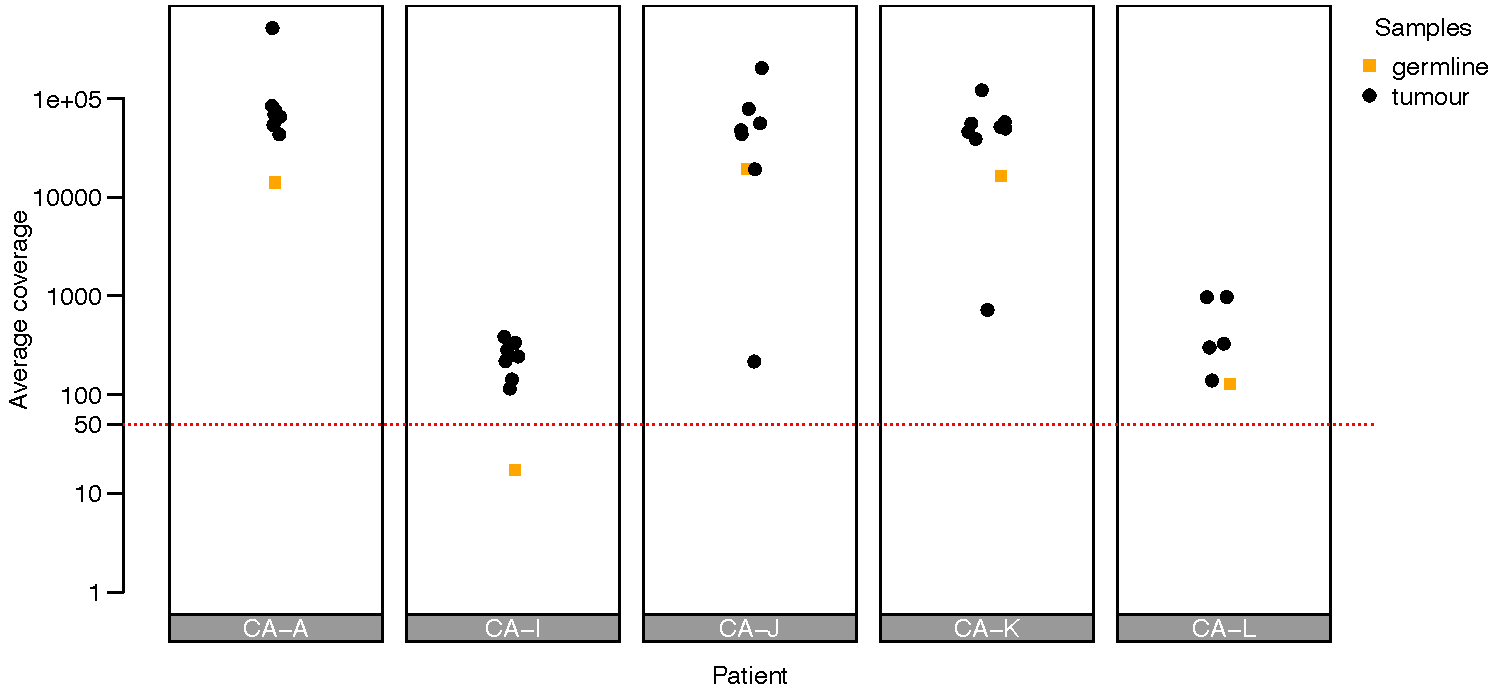
\includegraphics[width=.99\linewidth]{Figures/CASCADE/mito/mtCoverage}
\vspace{-1em}
\caption[Average coverage of mitochondrial DNA of CASCADE patients]{Average coverage of mitochondrial DNA of CASCADE patients: Orange squares show germline sample for each patient; black points show tumour samples; horizontal red dotted line shows quality cut off suggested by \protect\textcite{Ludwig2019}} \label{fig:mtCoverage}
\end{figure}

This shows, that even without specifically enriching for mitochondrial DNA, most samples will contain enough tumour reads for this analysis.

To ensure optimal results, we excluded all samples with an average coverage of less than 50x. This means we remove the germline sample for patient CA-I, however as we expect the germline sample to be the ancestral state for all samples, so it can be reconstructed. Secondly, we were more interested in the relation of tumour samples with each other, which is still possible.

In contrast to the simple hamming distance used for the presence-absence vector representation of canonical somatic variants (\autoref{cascade-sec:phylo}) for mitochondrial variants we employed a allele frequency ($vaf$) based distance (\autoref{eq:mitoDist}) of two samples~$s_i$ and $s_j$. The difference in read support is normalised with the product of the total allelic depth~$cov$ and summed up at all sites of variation~$v$.

\begin{equation}
mitoDist(s_i,s_j) = \sum_{v \in Variants} \left| \frac{vaf_{s_i}(v) \cdot cov_{s_i}(v) - vaf_{s_j}(v) \cdot cov_{s_j}(v)}{cov_{s_i}(v) \cdot cov_{s_j}(v)} \right| \label{eq:mitoDist}
\end{equation}
\myequation[\ref{eq:mitoDist}]{Mitochondrial variants based distance function of two samples}

This distance was only calculated for variant sites where both samples had at least a coverage of 100x to have a representative sampling of the allelic prevalence in each sample as a human cell usually has more than 100 mitochondria \cite{Cole2016}.


\subsection{Results}
\label{cascade-sec:mitoResults}
While the mitochondrial variants analysis only uses a fraction of the size of the genomic DNA loci and therefore most likely breaks the infinite sites assumption \cite{Kimura1969}, it was still able to generate a second viewing angle at the heterogeneity and trajectory of the multi-regional samples in each patient.

\subsubsection{Patient CA-A}

While the separation of progression ((11, 47, 55, and 59) and stable (26, 31, 41, and 57) disease sites was already visible in the somatic phylogeny, the bottle neck of treatment and new metastasis is more obvious in the mitochondrial phylogeny. However the individual resolution of splits appeared to be lower for the mitochondrial reconstruction (\autoref{fig:CA99mitoPhylo}).


\begin{figure}[h]
\centering
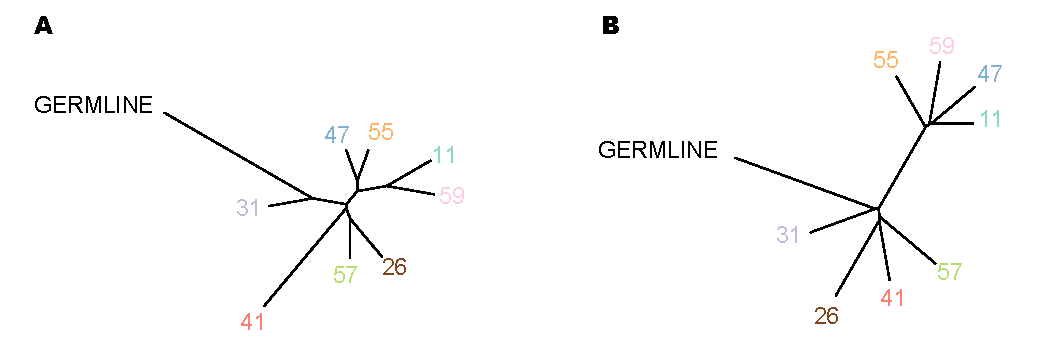
\includegraphics[width=.99\linewidth]{Figures/CASCADE/mito/CA99SomVsMitoPhylo.pdf}
\caption[Mitochondrial and somatic phylogenetic reconstruction of CA-A]{Mitochondrial and somatic phylogenetic reconstruction of CA-A: Somatic variants based reconstruction (A) and mitochondrial variants based reconstruction (B)} \label{fig:CA99mitoPhylo}
\end{figure}

\subsubsection{Patient CA-I}

Neither the somatic variants nor the mitochondrial variants resolved the evolutionary trajectory in a granular fashion. The slightly long stem of shared variants was most likely due to the low coverage of the germline sample. Similar to all other patients, the substructure of the samples was changed. While on the somatic variants showed sample 566 as the closest to the germline sample, mitochondrial variants instead indicated sample 559 as the closest (\Autoref{fig:mtCoverage,fig:CA51mitoPhylo}).


\begin{figure}[ht]
\centering
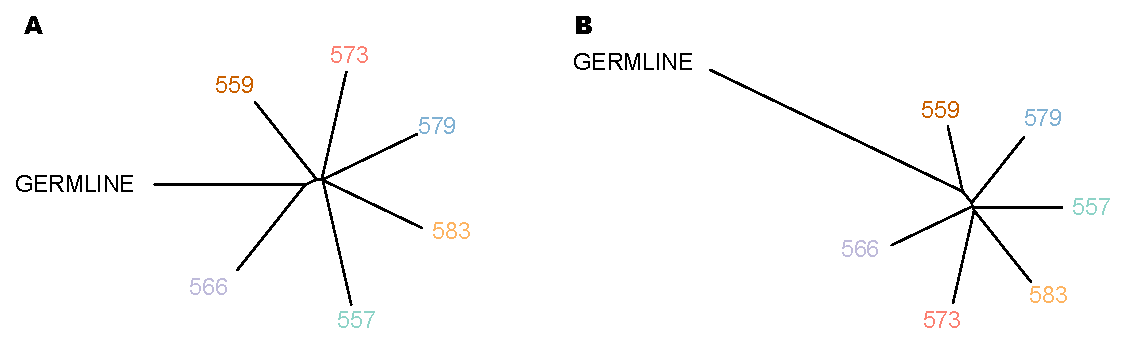
\includegraphics[width=.99\linewidth]{Figures/CASCADE/mito/CA51SomVsMitoPhylo.pdf}
\caption[Mitochondrial and somatic phylogenetic reconstruction of CA-I]{Mitochondrial and somatic phylogenetic reconstruction of CA-I: Somatic variants based reconstruction (A) and mitochondrial variants based reconstruction (B)} \label{fig:CA51mitoPhylo}
\end{figure}


\subsubsection{Patient CA-J}

In contrast to the somatic variant phylogeny, the mitochondrial reconstruction showed sample 2 as a substantial outlier and instead of the two samples 24 and 28 only sample 28 was grouped closely with the germline sample. The low distance to the germline sample can be attributed to its very low tumour purity. However sample 24, which was also evolutionary close to the germline sample when using somatic variants, is now grouped with the other samples with similar copy number profile, even due to the lower purity (\autoref{tab:ca80cnv}, \autoref{fig:CA80mitoPhylo})

\begin{figure}[ht]
\centering
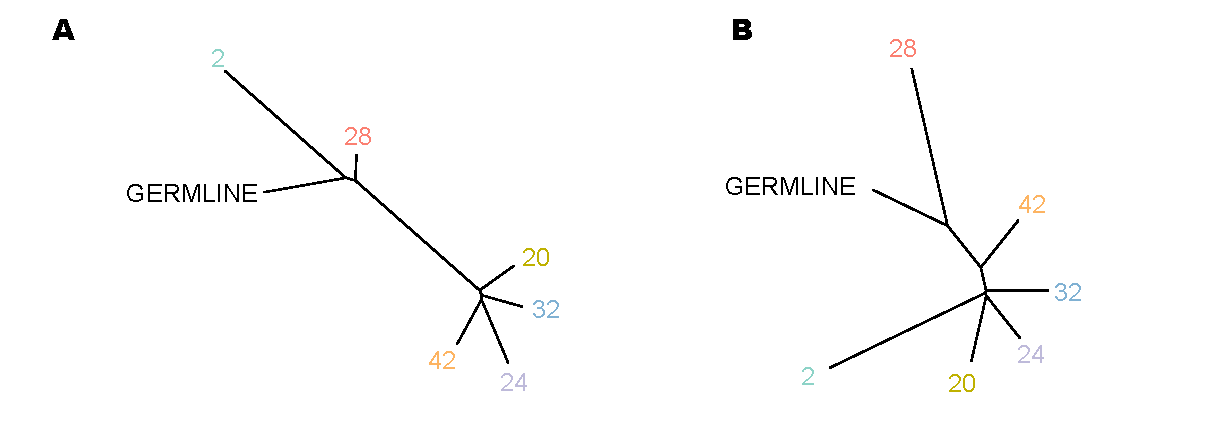
\includegraphics[width=.99\linewidth]{Figures/CASCADE/mito/CA80SomVsMitoPhylo.pdf}
\caption[Mitochondrial and somatic phylogenetic reconstruction of CA-J]{Mitochondrial and somatic phylogenetic reconstruction of CA-J: Somatic variants based reconstruction (A) and mitochondrial variants based reconstruction (B)} \label{fig:CA80mitoPhylo}
\end{figure}


\subsubsection{Patient CA-K}

In contrast to the somatic variant phylogeny, which showed a outgroup of samples 8 and 9, with a second cluster of samples 4, 5, and 6, the mitochondrial data supported a half way split into two groups. These groups almost perfectly split the samples into the left and right body half with sample 6 being the only sample from  the right side clustered with the left lung and brain samples 8, 9, and 13. These data suggested that while only samples 8 and 9 showed a whole genome duplication and the \textit{APC} ``stop gained`` mutation, they were closer related to the other samples than assumed from the somatic variant analysis (\autoref{tab:ca82cnv}, \Autoref{fig:ca82heatmap,fig:CA82mitoPhylo}).

\begin{figure}[ht]
\centering
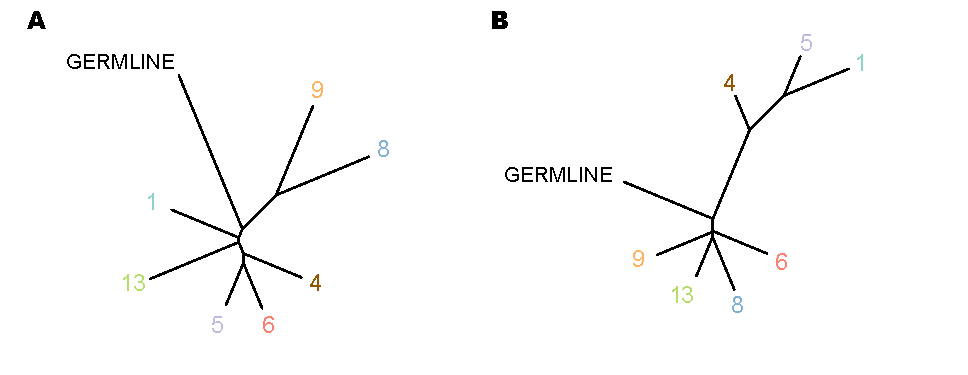
\includegraphics[width=.99\linewidth]{Figures/CASCADE/mito/CA82SomVsMitoPhylo.pdf}
\caption[Mitochondrial and somatic phylogenetic reconstruction of CA-K]{Mitochondrial and somatic phylogenetic reconstruction of CA-K: Somatic variants based reconstruction (A) and mitochondrial variants based reconstruction (B)} \label{fig:CA82mitoPhylo}
\end{figure}


\subsubsection{Patient CA-L}
While the somatic variants linked the small cell carcinoma samples P.1 and 8 together, the mitochondrial analysis shows that the closest relative to P.1 was P.2. as both of the Progression samples were taken 14 months ahead of the death of the patient, this fitted the clinical history of the samples better. Additionally instead of grouping the the adenocarcinoma sample 17A and 26 together, the mitochondrial phylogeny suggests, that while they share a common resistance mechanism (EGFR~T790M), it might have been acquired in parallel instead of being seeded from the same lesion, as all samples other than the P.1/2 samples are not grouped together. Lastly, the closeness of sample 8 and the germline sample possibly indicated a presence of small cell disease already ``before`` the progression samples. However the FFPE conservation of the P samples could have altered the molecular clock and influenced the branching site on the tree (\Autoref{fig:ca86heatmap,fig:CA86mitoPhylo}).

\begin{figure}[ht]
\centering
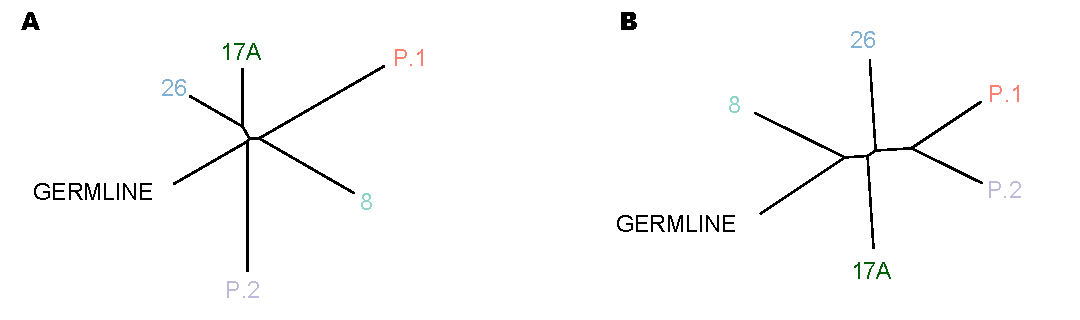
\includegraphics[width=.99\linewidth]{Figures/CASCADE/mito/CA86SomVsMitoPhylo.pdf}
\caption[Mitochondrial and somatic phylogenetic reconstruction of CA-L]{Mitochondrial and somatic phylogenetic reconstruction of CA-L: Somatic variants based reconstruction (A) and mitochondrial variants based reconstruction (B)} \label{fig:CA86mitoPhylo}
\end{figure}

\subsection{Summary}
With the analysis of the mitochondrial history of samples, we could shed some light on the timing of lesions and the development of resistance mechanisms, which is not heavily influenced by the treatment and its selection pressure. While the infinite sites hypothesis does not hold true for mitochondrial DNA, due to the limited sites and reduced repair mechanisms, the selection pressure of treatment and their resistance mechanisms parallel evolution biased the analysis of multiple related tumour sample when using somatic variants.

This method could offer an alternate view on the history of samples and their kinship with data that was previously discarded but was abundantly available at no extra cost. Ideally both somatic variants and mitochondrial variants would be integrated into a holistic approach, however due to the substantial difference in scale between nuclear DNA and mitochondrial DNA, the process is intricate and outside the scope of this work.